\documentclass[./main.tex]{subfiles}

\begin{document}

\section{Machine Learning Theory}\label{sec:theory}
Throughout this section the theory of machine learning that will be used in this thesis is described and explained. In Section \ref{subsec:motivation_theory} we describe the general motivation behind using machine learning. Then, in Section \ref{subsec:ml_paradigmes} we explain the three most common paradigms in machine learning and how we will use some of them. In Section \ref{subsec:evaluation} we give a brief overview of how to evaluate a developed model. Lastly, in Section \ref{subsec:NeuralNetworks} we describe the mathematics behind feedforward- and convolutional neural networks .

\subsection{Motivation}\label{subsec:motivation_theory}
It can be difficult for humans to recognize certain patterns and trends in data. This becomes more difficult the greater the quantity of the data is, which is becomming more and more common with the rapidly growing topic of \textit{Big Data}. For this reason, computers are often used instead of humans to recognize patterns and trends in the data by analyzing the data, which is what is called \textit{Machine Learning}. In this thesis, we will use machine learning in section \ref{experiement} to develop a model to estimate the 2D pose of a single human in an image. Later, in section \ref{sec:XAI}, we will use machine learning to improve our understanding of the model.

\subsection{Machine Learning Paradigms}\label{subsec:ml_paradigmes}
Machine learning is usally split into the following three paradigms
\begin{enumerate}
    \item \textit{Supervised learning} where the data consists of features and labels. By analyizing the data the algorithm learns to predict the labels given the features \cite{ESL}. Supervised learning is further split into \textit{classification} and \textit{regression}. If the value of each label is limited, then the task is a classification task. If the value of each label is not limited, then the task is a regression task. 
    \item \textit{Unsupervised learning} where the data only consists of features. The algorithm then learns properties of the data, without any provided labels \cite{ESL}.
    \item \textit{Reinforcement learning} where the algorithm learns to perform the action in a given environment that yields the highest reward \cite{PRML}.
\end{enumerate}
In this thesis we will make use of supervised learning when developing our model for pose estimation. Later, unsupervised learning is used when we explore our developed model.

\subsection{Evaluation of Machine Learning Models}\label{subsec:evaluation}
When developing a machine learning model it is important to know how trustworthy the developed model is. This is usually done by testing how good the model is at generalizing unseen data, which is done by making use of \textit{evaluation metrics}.

\subsubsection{Splitting the dataset}
When developing a machine learning model, the data needs to both create the model, but also to evaluate the model. For the evaluation of the model, one of the two following techniques is usually used

\begin{enumerate}
    \item \textit{Cross validation} where the data is split into $K$ random non-overlapping chunks of equal size. The model is then trained for $K$ rounds on $K - 1$ of the chunks, where the last chunk is used for evaluating the model. After each round the parameters of the model is reset to ensure one round does not affect another round. After the $K$ rounds the average loss of the $K$ rounds is the loss of the model \cite{MAD_book}.
    \item \textit{Train-validation-test} where the data is split into $3$ random non-overlapping chunks. The training dataset is then used for training the model and the validation dataset is used for evaluating the model as it is being developed - this often means, that the \textit{hyperparameters}, the paramters that are not possible to fit from the data, are being tweaked to yield the best validation loss. Lastly, the testing dataset is used as a final evaluation of the model to yield an unbiased evaluation of the model. Once the testing dataset has been used it can no longer be used for evaluating the data, as this ensure an unbiased evaluation \cite{MAD_L3}.
\end{enumerate}
Throughout this thesis the train-validation-test technique will be used over cross validation for evaluating the developed models. This is done, since cross validation is better suited for smaller datasets, as the runtime is much greater than the runtime of the train-validation-test technique.

\subsubsection{Evaluation Metrics for Supervised Machine Learning (Loss Functions)}
When we have trained a model, we need to somehow evaluate how well the model performs on unseen data. This is usually done by making use of evaluation metrics or \textit{loss functions}. There are many different loss functions, each with their own advantages and disadvantages. One of the most common loss functions for regression is the \textit{Mean Squared Error (MSE)}, defined as
$$MSE = \frac{1}{n} \sum_{i = 1} ^n \left( y_i - \hat{y}_i \right)^2$$
where $y_i$ is the true value of the $i$th observation and $\hat{y}_i$ is the estimated value of the $i$th observation. Thus, $MSE$ measures the average squared difference between the true observation and the estimated observation. The aim of a model is thus to make the $MSE$ as small as possible \cite{ISL}.

\subsection{Neural Networks} \label{subsec:NeuralNetworks}
In recent years \textit{deep learning} and \textit{neural networks} have revolutionized the use of machine learning. In this thesis a neural network will be used for performing the human pose estimation. Throughout subsection \ref{subsec:NeuralNetworks} the theory and mathematics behind neural networks is described and explained.
\subsubsection{Feedforward Neural Networks} \label{subsubsec:FeedforwardNN}
\begin{algorithm}[htbp]
    \caption{GradientDescent \cite{d2l}}
    \label{Algorithm:gradient_descent_alg}
    \begin{algorithmic}[1]
        \Require Learning rate $\eta$
        \Require Starting position $\bm{\theta}$
        \Require Function to minimize $f$
        \While{stopping criterion not met}
            \State Apply update: $\bm{\theta} = \bm{\theta} - \eta \nabla f(\bm{\theta})$
        \EndWhile
        \State \textbf{return} $\bm{\theta}$
    \end{algorithmic}
\end{algorithm}
\noindent \textbf{Overfitting and Regularization} \\
% Lidt uenig med definitionen af overfitting - taget fra DeepLearning. Tænk på underfitting.
The main goal of a machine learning model is to generalize well on unseen data. This can often be difficult, as the model simply "remembers" the training data instead of learning the patterns in the training data. In other words, the gap between the training error and the test error is too large, which is a concept called \textit{overfitting}. Certain techniques are designed to reduce the test error - these techniques are collectively called \textit{regurlization} \cite{DeepLearning}. 
\\
\\
\textbf{Gradient Descent} \\
The goal of a machine learning model when training is to minimize its loss. There are different methods to do so, however, the most common algorithms are variants of \textit{gradient descent}, whose algorithm is described in Algorithm \ref{Algorithm:gradient_descent_alg}. The algorithm works by taking a learning rate $\eta$, a starting position $\bm{\theta}$ and a function $f$ as input, where $f$ is the function to minimize. It then computes the gradient of $f$ with respect to $\bm{\theta}$, and subtracts the gradient times $\eta$ from $\bm{\theta}$. This is done untill a stopping condition is met, such as when the magnitude of the gradient $\left| \nabla f(\bm{\theta}) \right|$ is small or untill a maximum amount of iterations has been reached \cite{d2l}.
\begin{figure}
    \centering
    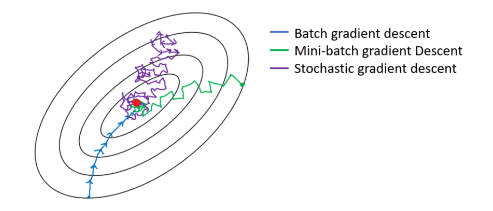
\includegraphics[width = 8 cm]{entities/batch_methods.PNG}
    \caption{Comparison of batch, mini-batch and stochastic gradient descent \cite{EML_optimization}}
    \label{fig:batch_methods}
\end{figure}
\\
\\
\noindent \textbf{Online, Mini-batch and Batch methods} \\
\noindent When gradient descent is used in machine learning, computing $\nabla f(\bm{x})$ is usually done by averaging the gradient of each of the $n$ observations of the trainingset, which is called a \textit{batch gradient method} and is computational inefficient, as the cost is $\mathcal{O}(n)$. It is therefore common to use variants of gradient descents, that reduces the cost of computing the gradient. In \textit{online gradient methods} (also known as \textit{stochastic gradient descent}) a single observation from the dataset is used to compute the gradient, which brings the cost down to $\mathcal{O}(1)$. In \textit{mini-batch gradient methods} a subset of the dataset is used to compute the gradient, making the cost $\mathcal{O}(|\mathcal{B}|)$, where $|\mathcal{B}|$ is the mini-batch size \cite{d2l}. \\
Choosing the right batch size can be difficult, however, there are a few guidelines which one can follow \cite{EML_optimization} \cite{d2l}
\begin{enumerate}
    \item Looking at Figure \ref{fig:batch_methods} we see, that batch gradient descent uses the fewest iterations, however, each iteration takes the longest to compute. On the other hand, in online gradient descent each iteration is the fastest to compute, however, it is also the method that uses the most iterations. Lastly, mini-batch gradient descent combines the two: it uses less iterations than online gradient descent, but more than batch gradient descent, and each iteration takes less time than in the case with batch gradient descent, but longer than in the case with online gradient descent.
    \item A batch size that is of power of $2$ can offer in better runtime for some hardware. A batch size that is often used for larger models is $16$, however, they typically range between $32$ and $256$.
    \item Smaller batch sizes can offer a regularizing effect, as it is difficult for the model to "remember" the complete dataset from batches that does not represent the whole dataset.
\end{enumerate}
\begin{algorithm}[htbp]
    \caption{RMSProp \cite{DeepLearning}}
    \label{Algorithm:RMSProp}
    \begin{algorithmic}[1]
        \Require Learning rate $\eta$
        \Require Decay rate $\rho$
        \Require Starting position $\bm{\theta}$
        \Require Small constant $\delta$, usually $10^{-6}$
        \Require Loss function $L$
        \Require Function to minimize $f$
        \State Initialize accumulation variables $\bm{r} = \bm{0}$
        \While{stopping criterion not met}
            \State \begin{varwidth}[t]{\linewidth}
            Sample a minibatch of $m$ observations from the training set $\{\bm{x}^{(1)}, ..., \bm{x}^{(m)}\}$ with corresponding targets $\bm{y}^{(i)}$
            \end{varwidth}
            \State Compute gradient: $\bm{g} = \frac{1}{m} \nabla_{\bm{\theta}} \sum_i L(f(\bm{x}^{(i)}; \bm{\theta}), \bm{y}^{(i)})$
            \State Accumulate squared gradient: $\bm{r} = \rho \bm{r} + (1 - \rho) \bm{g} \odot \bm{g}$
            \State Compute parameter update: $\Delta\bm{\theta} = - \frac{\eta}{\sqrt{\delta + \bm{r}}} \odot \bm{g}$
            \State Apply update: $\bm{\theta} = \bm{\theta} + \Delta \bm{\theta}$ 
        \EndWhile
        \State \textbf{return} $\bm{\theta}$
    \end{algorithmic}
\end{algorithm}
\noindent \textbf{Optimization Algorithms} \\
\noindent Online, mini-batch and batch gradient descent are all optimization algorithms used for estimating the minimum of a function. One problem of these algorithms is, that the learning rate can be difficult to choose. Therefore, there have been developed a range of various optimization algorithms that uses a separate learning rate for each parameter and automatically adapt these learning rates. One of which is \texttt{RMSProp}, which has been visualized in Algorithm \ref{Algorithm:RMSProp}. The algorithm works by using an decaying average that discards knowledge from the past, so that it can converge after finding a convex bowl. The algorithm uses a hyperparameter $\rho$, that controls the length scale of the moving average \cite{DeepLearning}.
\\
\\
\textbf{Batch Normalization} \\
\textit{Batch normalization} is a reparametrization method, which is applied to individual layers. If $\bm{x} \in \mathcal{B}$ is an input to the batch normalization, $\text{BN}$, then batch normalization is done by the following
$$\text{BN}(\bm{x}) = \bm{\gamma} \odot \frac{\bm{x} - \hat{\bm{\mu}}_{\mathcal{B}}}{\hat{\bm{\sigma}}_{\mathcal{B}}} + \bm{\beta}$$
where
$$\hat{\bm{\mu}} = \frac{1}{|\mathcal{B}|} \sum_{i} \mathcal{B}_i$$
and
$$\hat{\bm{\sigma}} = \sqrt{\epsilon + \frac{1}{|\mathcal{B}|} \sum_{i} \left(\mathcal{B} - \bm{\mu} \right)_i ^2 },$$
which makes the minibatch have $0$ mean and unit variance. $\bm{\gamma}$ and $\bm{\beta}$ are then used to make the mini-batch have an arbitrary mean and standard deviation and are two parameters that needs to be learned when the network is being fitted. This helps the network to converge, as the batch normalization keeps centering the mean and standard deviation of the mini-batches \cite{d2l}.
\\
\\
\textbf{Epoch} \\
An \textit{epoch} is an iteration through the whole dataset during fitting of the network. Multiple epochs are often needed to reach the minimum of the loss function \cite{d2l}.
\\
\begin{figure}[htbp]
    \centering
    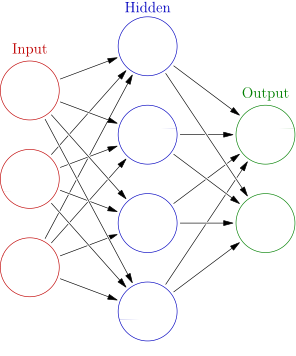
\includegraphics[height = 5 cm]{entities/feed_forward_nn.jpg}
    \caption{Visualization of a feedforward neural network with a single hidden layer \cite{feedforward_nn}}
    \label{feedforward_nn}
\end{figure}
\\
\noindent \textbf{The Architecture and Forwardpropagation} \\
One of the most common types of neural networks are \textit{feedforward neural networks}, where the data flows unidirectionally through the network. Such a network is visualized in Figure \ref{feedforward_nn}. The network is built up of three types of components: the \textit{input layer}, the \textit{hidden layers} and the \textit{output layer}. Each layer is built up of \textit{units}, also called \textit{neurons} (which are visualized as circles in Figure \ref{feedforward_nn}), where each neuron has a \textit{bias} assigned to it, and is connected to one or two other layers through \textit{edges} (which are visualized as arrows in Figure \ref{feedforward_nn}), where each edge has a \textit{weight} assigned to it. Hidden layers are connected to two other layers - one before the hidden layer and one after the hidden layer - where the input layer is only connected to the next layer in the network and the output layer is only connected to the previous layer in the network. \\
We can define the network mathemaically by letting $a_n ^{(i)}$ denote the value of the $n$th node in the $i$th layer, $w_{m, n}$ denote the value of the weight of the edge connecting the $n$th node in the $i$th layer to the $m$th node in layer $i + 1$ and $b_n ^{(i)}$ denote the bias corresponding to the $n$th node in the $i$th layer. \\
When data flows through the model it follows the following formula
$$\bm{a}^{(i + 1)} = g^{(i + 1)} \left( \bm{z}^{(i + 1)} \right)$$
where
$$\bm{z}^{(i + 1)} = \bm{W}^{(i + 1)} \bm{a}^{(i)} + \bm{b}^{(i + 1)},$$
$\bm{W}^{(i + 1)}$ is the weights between layer $i$ and layer $i + 1$ defined by
\begin{center}
    \begin{math}
        \bm{W}^{(i + 1)} =
        \begin{pmatrix}
            w_{0, 0} & w_{0, 1} & \cdots & w_{0, n} \\
            w_{1, 0} & w_{1, 1} & \cdots & w_{1, n} \\
            \vdots & \vdots & \ddots & \vdots \\
            w_{m, 0} & w_{m, 1} & \cdots & w_{m, n}
        \end{pmatrix}
        ,
    \end{math}
\end{center}
$\bm{a}^{(i)}$ is the values of the nodes in the $i$th layer defined by
\begin{center}
    \begin{math}
        \bm{a}^{(i)} =
        \begin{pmatrix}
            a_{0} ^{(i)} \\
            a_{1} ^{(i)} \\
            \vdots \\
            a_{n} ^{(i)} \\
        \end{pmatrix}
        ,
    \end{math}
\end{center}
$\bm{b}^{(i + 1)}$ is the values of the biases of layer $i + 1$ defined by
\begin{center}
    \begin{math}
        \bm{b}^{(i + 1)} =
        \begin{pmatrix}
            b_{0} ^{(i + 1)} \\
            b_{1} ^{(i + 1)} \\
            \vdots \\
            b_{m} ^{(i + 1)} \\
        \end{pmatrix}
    \end{math}
\end{center}
and $g$ is an \textit{activation function}, that is typically applied element-wise \cite{DeepLearning} \cite{3b1b_1}. One often used activation function is the \textit{rectified linear activation function} (or \textit{ReLU} for short) defined by
$$g(x) = \max\{0, x\}.$$
The ReLU-function is very close to being linear, making the function keep many of the properties of linear functions that make them easy to optimize and generalizing, which are two great advantages of using the ReLU-function. Another great advantage of using the ReLU-function is stated by the \textit{universal approximation theorem} which states, that a feedforward network with a linear output layer and at least one hidden layer with the ReLU-function (or another activation function from a wide class of activation functions) can approximate any continuous function on a closed and bounded subset of $\mathbb{R}^n$ (and actually some functions outside of this class), as long as the network has enough hidden neurons \cite{DeepLearning}. 
\\
\\
\noindent \textbf{Backpropagation} \\
Backpropagation is an algorithm used to compute the gradient of the network. It is used together with an optimization algorithm, such as \texttt{RMSProp}, to train the model by minimizing the training loss of the model. Backpropagation happens after data has flowed through the model from the input to the output, and works by computing the gradient of each parameter sequentially from the output to the input of the model. The procedure makes heavily use of the \textit{chain rule} from calculus, which states, that if we let $\bm{x} \in \mathbb{R}^m$, $\bm{y} \in \mathbb{R}^n$, $g$ be a function that maps from $\mathbb{R}^m$ to $\mathbb{R}^n$ and $f$ be a function that maps from $\mathbb{R}^n$ to $\mathbb{R}$, then, if we let $\bm{y} = g(\bm{x})$ and $z = f(\bm{y})$, we can then compute $\frac{\partial z}{\partial x_i}$ by
$$\frac{\partial z}{\partial x_i} = \sum_j \frac{\partial z}{\partial y_j} \frac{y_j}{x_i}$$
\cite{DeepLearning}. If we use this to find the gradient of each parameter, we will find, that the partial derivative for each weight is
$$\frac{\partial L}{\partial w_{jk} ^{(i)}} = \frac{\partial z_j ^{(i)}}{\partial w_{jk} ^{(i)}} \frac{\partial a_j ^{(i)}}{\partial z_j ^{(i)}} \frac{\partial L}{\partial a_j ^{(i)}} = a_k ^{(i - 1)} g ^{\prime (i)} \left( z_j ^{(i)} \right) \frac{\partial L}{\partial a_j ^{(i)}}$$
and the partial derivative of each bias is
$$\frac{\partial L}{\partial b^{(i)} _j} = \frac{\partial z^{(i)} _j}{\partial b^{(i)} _j} \frac{\partial a_j ^{(i)}}{\partial z^{(i)} _j} \frac{\partial L}{\partial a_j ^{(i)}} = g^{\prime (i)} \left( z_j ^{(i)} \right) \frac{\partial L}{\partial a_j ^{(i)}}$$
where for both cases
$$ \frac{\partial L}{\partial a_j ^{(i)}} = \sum_{j = 0} ^{n_i - 1} w_{jk} ^{(i + 1)} g^{\prime (i + 1)} \left( z_j ^{(i + 1)} \right) \frac{\partial L}{\partial a_j ^{(i + 1)}}.$$
if $\bm{a}^{(i)}$ is not the output-layer. Once the partial derivative of all weights and biases has been found, the gradient vector can be formed and an optimization method can be used to optimize the parameters of the model \cite{3b1b_4}.


\subsubsection{Convolutional Neural Networks} \label{subsubsec:CNN}
\begin{figure}[htbp]
    \centering
    \begin{subfigure}[t]{0.4\textwidth}
        \centering
        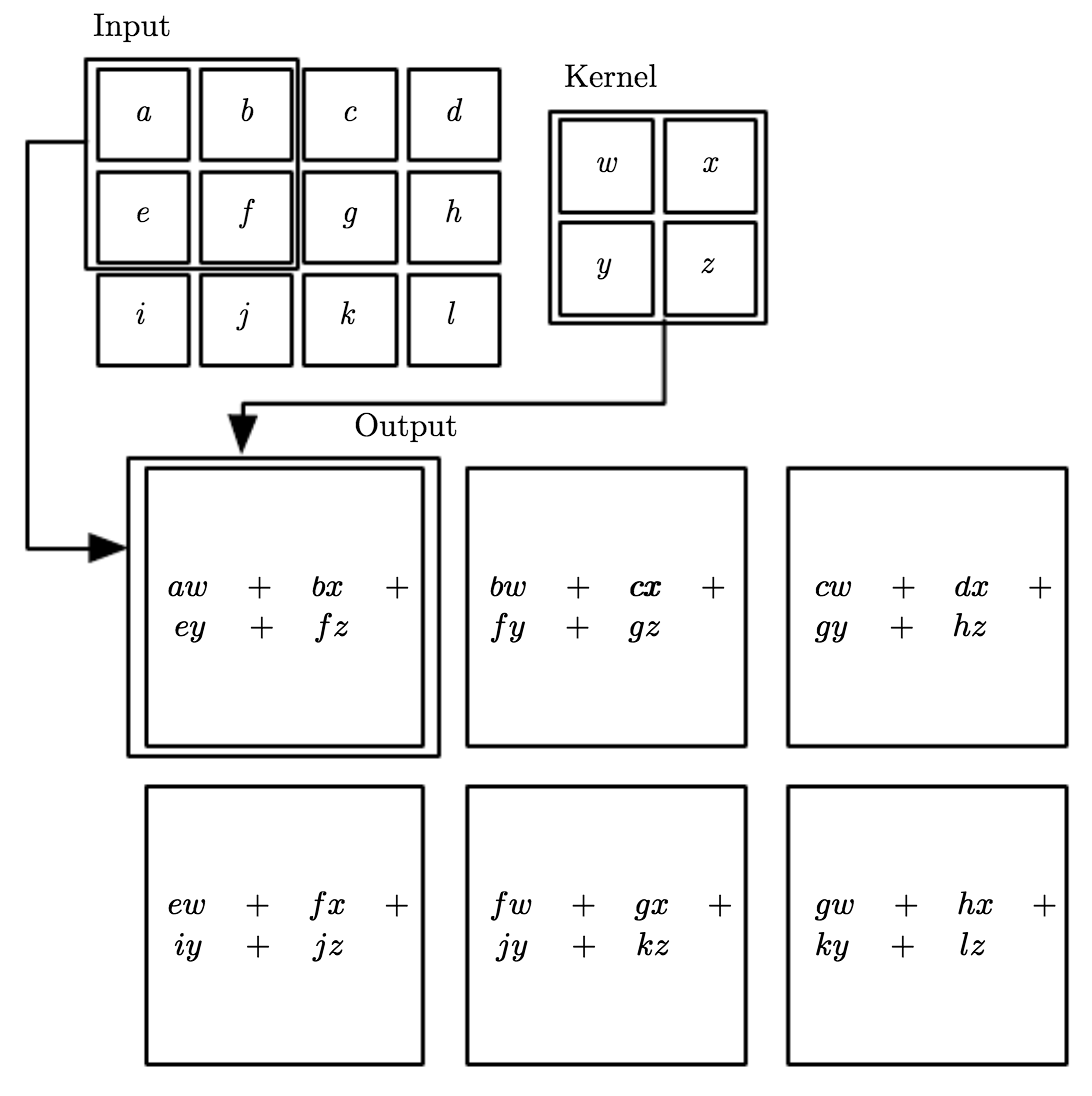
\includegraphics[height = 6 cm]{entities/2d_convolution_example.png}
        \caption{Example of a 2D convolution \cite{DeepLearning}}
    \end{subfigure}
    \begin{subfigure}[t]{0.4\textwidth}
        \centering
        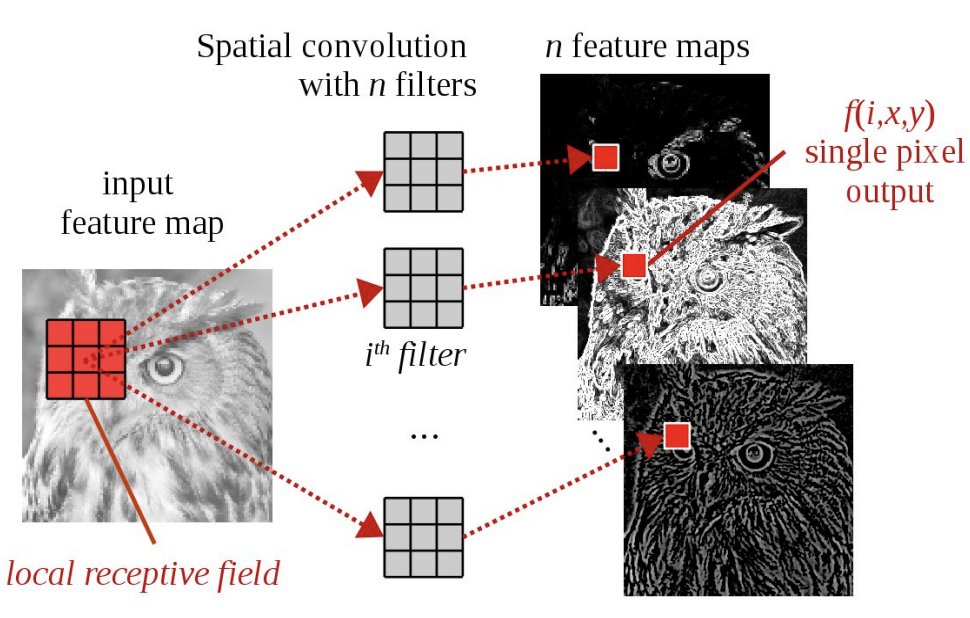
\includegraphics[height = 5 cm]{entities/3d_convolution_example.png}
        \caption{Example of a convolution with multiple filters \cite{Everything}}
    \end{subfigure}
    \caption{Convolutions visualized}
    \label{fig:convolutionexample}
\end{figure}
Feedforward neural networks introduced in \ref{subsubsec:FeedforwardNN} can be used for pattern recognition within images, however, they are usually not used for this task. Consider a colored input image of dimension $64 \times 64$. If we were to use a feedforward neural network on this image, each neuron in the first hidden layer would be connected to the input layer through $12.288$ weights. Not only would this use a lot of computational power and time to train, however, a network of this size would also be prone to overfitting. Instead, \textit{convolutional neural networks} (also known as \text{CNN}'s) are usually used. A CNN usually consists of \textit{convolutional layers}, \textit{pooling layers} and \textit{fully-connected layers}, where the fully-connected layers are analogous to the layers in a feedforward neural network \cite{CNN}.
\\
\\
\textbf{Convolutional layers} \\
A convolutional layer is composed of a set of \textit{kernels} (also known as \textit{filters}), which are matrices of weights of dimension $k \times k$, where $k$ usually is $5$, $3$ or $1$, and each weight is a parameter for the model to be learned \cite{Everything}. Each kernel is used on the input to produce a \textit{feature map}. The kernels are applied to the input by "sliding" over the input (where the step size is called \textit{stride} and is usually by default equal to $1$). Each $k \times k$ grid of the input (called the \textit{local receptive field}) is then used to compute the dot-product between the grid and each kernel, which is then placed in the corresponding feature map of each kernel, as visualized in Figure \ref{fig:convolutionexample}. When all of the feature maps have been computed, the feature maps are stacked together, forming a tensor, which is then returned by the layer and a activation function can be applied. \\
As described previously, by using a convolutional layer we can dramatically decrease the amount of weights used by the layer. If we were to use a $3 \times 3$ kernel on a colored image, we would reduce the amount of weights on each neuron in the following layer from $12.288$ down to just $27$, reducing both the training time and making the network less prone to overfitting \cite{CNN}.
\\
\\
\textbf{Pooling layers} \\
Pooling layers are layers used to reduce the dimension of the input. The most common pooling layer is the \textit{maxpooling}-operation. The operation works by considering each $k \times k$ grid, like in the case with the convolutional layer, in which the maximum entry in that grid is being inserted into the output \cite{CNN}.
\\
\\
\textbf{Nearest Neighbour Upsampling} \\
\begin{algorithm}[htbp]
    \caption{Nearest Neighbour Upsampling \cite{NNUpsampling}}
    \label{Algorithm:NNUpsampling}
    \begin{algorithmic}[1]
        \Require Input image $X$ of size $m \times n$
        \Require Wanted output size $xm \times yn$
        \State Create empty image $O$ of size $xm \times yn$
        \ForAll{pixel, $p$, in $X$}
            \State $i,j = \text{index of } p \text{ in } X$
            \State Insert $p$ at index $(xi, yj)$ in $O$
        \EndFor
        \ForAll{empty pixel $p \in O$}
            \State Let $p$ be the value of the nearest neighbour
        \EndFor
        \State \textbf{return} $O$
    \end{algorithmic}
\end{algorithm}
Sometimes we want to increase the size of an image. This is done by making use of \textit{upsampling} (also known as \textit{interpolation}) techniques. One of the most common upsampling techniques is \textit{nearest neighbour upsampling}, whose pseudocode has been written in \ref{Algorithm:NNUpsampling}. The algorithm starts off by taking an image, $X$, of size $m \times n$, as input, which we wish to upsample to size $xm \times yn$. The algorithm then loops over each pixel, $p$, in $X$, finds the corresponding index, $i, j$, of $p$ in $X$, and places $p$ at index $(xi, yj)$ in the output image $O$ of size $xm \times yn$. When this is done, it assigns each of the empty pixel in $O$ the value of their nearest neighbour, making each pixel in $O$ have a value, and then returns $O$ \cite{NNUpsampling}.

\end{document}